\chapter{Numerics}
\section{Finite Difference Method - FDM}
\subsection{First Order Derevative}
For arbitraty number of points one can find
%----------------------------------------------------------------
\begin{equation}
	\label{eqn:diff_gen}
    \left.\pdv{f}{x_i} \right|_0 \approx \frac{\sum_{n = 1}^N \frac{f_n - f_0}{\vec{x}_{n, i} - \vec{x}_{0, i}} \cdot w_n \cdot N}{\sum_{n=1}^N w_n}
\end{equation}
%----------------------------------------------------------------
substituting
%----------------------------------------------------------------
\begin{subequations}
	\begin{align}
		\label{eqn:subs}
		\vec{r}_{n, i} &\equiv \vec{x}_{n, i} - \vec{x}_{0, i} \\
		\hat{w}_n &\equiv \frac{w_n \cdot N}{\sum_{n=1}^N w_n} \\
		q_{n, i} &\equiv  \frac{\hat{w}}{\vec{r}_{n, i}}
	\end{align}
\end{subequations}
%----------------------------------------------------------------
where $w_n$ is a weighting function wich is invesly proportional to the distance between the origin $\vec{x}_0$ and the evlauted point $\vec{x}_n$
%----------------------------------------------------------------
\begin{equation}
	w_n \propto \frac{1}{|\vec{r}_{n}|}.
\end{equation}
%----------------------------------------------------------------
Substituting Eqn.~(\ref{eqn:subs}) in Eqn.~(\ref{eqn:diff_gen}) leads to
\begin{equation}
	\left.\pdv{f}{x_i} \right|_0 \approx \sum_{n = 1}^N (f_n - f_0) \cdot q_{n, i} = \sum_{n = 1}^N f_n \cdot q_{n, i} - f_0 \cdot \underbrace{\sum_{n = 1}^N q_{n, i}}_{Q_i}
\end{equation}
%----------------------------------------------------------------
\begin{equation}
	\label{eqn:diff}
	\left.\pdv{f}{x_i} \right|_0 \approx \sum_{n = 1}^N f_n \cdot q_{n, i} - f_0 \cdot Q_i
\end{equation}
%----------------------------------------------------------------

\subsection{$q$-Order Derevative}
The $q$-order derevative of a scalar function $f$ can be approximated similar Eqn.~(\ref{eqn:diff}) to as
%----------------------------------------------------------------
\begin{equation}
	\left.\pdv[q]{f}{x_i}\right|_0 \approx \sum_{n = 1}^N \left.\pdv[q-1]{f}{x_i} \right|_n \cdot q_{n, i} - \left.\pdv[q-1]{f}{x_i} \right|_0  \cdot Q_i
\end{equation}
%----------------------------------------------------------------
or more compact
%----------------------------------------------------------------
\begin{equation}
	\left.\pdv[q]{f}{x_i}\right|_0 \approx \sum_{n = 1}^N f^{(q-1)}_{n, i} \cdot q_{n, i} - f^{(q-1)}_{0, i}  \cdot Q_i
\end{equation}
%----------------------------------------------------------------

\subsection{Laplace Operator}
The Laplace Operator is defined for cartasian coordinates as
%----------------------------------------------------------------
\begin{equation}
	\nabla^2 f = \sum_{i = 3}^3 \pdv[2]{f}{x_i}
\end{equation}
%----------------------------------------------------------------
for derivation second order can be defineds as
%----------------------------------------------------------------
\begin{equation}
	\label{eqn:laplace}
	\left.\pdv[2]{f}{x_i}\right|_0 \approx \sum_{n = 1}^N \left.\pdv{f}{x_i} \right|_n \cdot q_{n, i} - \left.\pdv{f}{x_i} \right|_0  \cdot Q_i
\end{equation}
%----------------------------------------------------------------
In Eqn.~(\ref{eqn:laplace}) $f'_0$ is defined as in Eqn~(\ref{eqn:diff}).
$f'_n$ is defined as
%----------------------------------------------------------------
\begin{equation}
	\left.\pdv{f}{x_i} \right|_n = f'_{n, i} \approx \frac{f_0 - f_n}{-\vec{r}_{n, i}} = \frac{fn - f_0}{\vec{r}_{n, i}}
\end{equation}
%----------------------------------------------------------------
combining leads to
%----------------------------------------------------------------
\begin{align}
	\left.\pdv[2]{f}{x_i}\right|_0 &\approx \sum_{n = 1}^N \frac{fn - f_0}{\vec{r}_{n, i}} \cdot q_{n, i} - \left( \sum_{n = 1}^N f_n \cdot q_{n, i} - f_0 \cdot Q_i \right) \cdot Q_i \\
	&= \sum_{n = 1}^N f_n \cdot q_{n, i} \cdot \frac{1}{\vec{r}_{n, i}} - f_0 \cdot \underbrace{\sum_{n = 1}^N  \frac{q_{n, i}}{\vec{r}_{n, i}}}_{\hat{Q}_i} - \sum_{n = 1}^N f_n \cdot q_{n, i} \cdot Q_i + f_0 \cdot Q_i^2
\end{align}
%----------------------------------------------------------------
which leads in the end to equation
%----------------------------------------------------------------
\begin{equation}
	\left.\pdv[2]{f}{x_i}\right|_0 \approx \sum_{n = 1}^N f_n \cdot q_{n, i} \cdot \left( \frac{1}{\vec{r}_{n, i}} - Q_i \right) + f_0 \cdot \left( Q_i^2 - \hat{Q}_i \right).
\end{equation}
%----------------------------------------------------------------
The equations above can be combined to the whole cartesian Laplace-Operator for $D$ dimensions
%----------------------------------------------------------------
\begin{equation}
	\nabla^2 f \approx \sum_{i = 1}^D \left[ \sum_{n = 1}^N f_n \cdot q_{n, i} \cdot \left( \frac{1}{\vec{r}_{n, i}} - Q_i \right) + f_0 \cdot \left( Q_i^2 - \hat{Q}_i \right) \right]
\end{equation}
%----------------------------------------------------------------
restructured (does it work like this??)
%----------------------------------------------------------------
\begin{equation}
	\nabla^2 f \approx \sum_{n = 1}^N f_n \left[ \sum_{i = 1}^D q_{n, i} \cdot \left( \frac{1}{\vec{r}_{n, i}} - Q_i \right) \right] + f_0 \cdot \sum_{i = 1}^D \left( Q_i^2 - \hat{Q}_i \right)
\end{equation}
%----------------------------------------------------------------

\subsubsection{Example - Heat Transfer in a Rod}
Equation
%----------------------------------------------------------------
\begin{equation}
	\pdv[2]{T}{x} = 0
\end{equation}
%----------------------------------------------------------------
the simulation set up can be seen in Fig.~(\ref{fig:rod_heat_transfer}).
%----------------------------------------------------------------
\begin{figure}[ht]
    \label{fig:rod_heat_transfer}
    \centering
    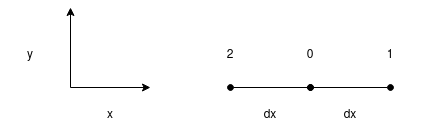
\includegraphics[width=0.8\linewidth]{rod.png}
    \caption{Test}
\end{figure}
%----------------------------------------------------------------
with the values
%----------------------------------------------------------------
\begin{table}[ht]
	\centering
    \caption{Simulation domain, rotational symmetry}
    \begin{tabular}{ccc}
    	\hline
    	$\Delta x / \si{\meter}$ & $T_1 / \si{\kelvin}$ & $T_2 / \si{\kelvin}$ \\
    	\hline\hline
    	\num{1} & \num{100} &\num{300} \\
    	\hline
    \end{tabular}
\end{table}
%----------------------------------------------------------------
this leads to the values
%----------------------------------------------------------------
\begin{table}[ht]
	\centering
    \caption{Simulation domain, rotational symmetry}
    \begin{tabular}{ccccccc}
    	\hline
    	$r_{n, 1}$ & $\hat{w}_n$ & $N$ & $\hat{r}_{1, 1}$ & $\hat{r}_{2, 1}$ & $q_{1, 1}$ & $q_{2, 1}$\\
    	\hline\hline
    	\num{1} & $1$ & \num{2} & \num{1} & \num{-1} & $1$ & $-1$ \\
    	\hline
    \end{tabular}
\end{table}
%----------------------------------------------------------------
leads to
%----------------------------------------------------------------
\begin{equation}
	Q_1 = q_{1, 1} + q_{2, 1} = 1 - 1 = 0
\end{equation}
%----------------------------------------------------------------
%----------------------------------------------------------------
\begin{equation}
	\hat{Q}_1 = \frac{q_{1, 1}}{\vec{r}_{1, 1}} + \frac{q_{2, 1}}{\vec{r}_{2, 1}} = 1 + 1 = 2
\end{equation}
%----------------------------------------------------------------
leads to
\begin{equation}
	\pdv[2]{T}{x} = \sum_{n = 1}^N f_n \cdot q_{n, 1} \cdot \left( \frac{1}{\vec{r}_{n, 1}} - Q_1 \right) + f_0 \cdot \left( Q_1^2 - \hat{Q}_1 \right)
\end{equation}
\begin{equation}
	\pdv[2]{T}{x} = f_1  +  f_2  - f_0 \cdot 2 = 0
\end{equation}
\begin{equation}
	100  +  300  - 2 \cdot f_0 = 0
\end{equation}
\begin{equation}
	f_0 = 200
\end{equation}

\subsection{Laplace-Operator with inhomogene pre-factor}
Assuming a Lpalce-Operator of the form
%----------------------------------------------------------------
\begin{equation}
	\alpha(n) \cdot \nabla^2 f
\end{equation}
%----------------------------------------------------------------
where $\alpha$ is defined as
%----------------------------------------------------------------
\begin{equation}
	\alpha(k) =
	\begin{cases}
		\alpha_0, & 0 < n < a_0 \\
		\alpha_1, & a_0 < n < (a_0 + a_1) \\
		\alpha_2, & (a_0 + a_1) < n < (a_0 + a_1 + a_2) \\
		& \vdots \\
		\alpha_N, & \sum_{i = 0}^{N - 1} a_i < n < \sum_{i = 0}^{N} a_i
	\end{cases}
\end{equation}
%----------------------------------------------------------------
where $n$ is the cell index and $a_i$ is the range of cells which are asigned the factor $\alpha_i$.
Writing with the assumption that every cell has its own value
%----------------------------------------------------------------
\begin{align}
	\left. \alpha_n \cdot \pdv[2]{f}{x_i}\right|_0 &\approx \sum_{n = 1}^N (f'_n - f'_0) \cdot q_{n, i} \cdot \alpha_n = \sum_{n = 1}^N f'_n \cdot q_{n, i} \cdot \alpha_n  - f'_0 \cdot \underbrace{\sum_{n = 1}^N q_{n, i} \cdot \alpha_n }_{A_i} \\
  &= \sum_{n = 1}^N \frac{fn - f_0}{\vec{r}_{n, i}} \cdot q_{n, i} \cdot \alpha_n  - \left( \sum_{n = 1}^N f_n \cdot q_{n, i} - f_0 \cdot Q_i \right) \cdot A_i \\
	&= \sum_{n = 1}^N f_n \cdot \frac{q_{n, i}}{\vec{r}_{n, i}} \cdot \alpha_n - f_0 \cdot \underbrace{\sum_{n = 1}^N  \frac{q_{n, i}}{\vec{r}_{n, i}}\cdot \alpha_n }_{\hat{A}_i} - \sum_{n = 1}^N f_n \cdot q_{n, i} \cdot A_i + f_0 \cdot Q_i \cdot A_i \\
	&= \sum_{n = 1}^N f_n \cdot q_{n, i} \cdot \left(\frac{\alpha_n}{\vec{r}_{n, i}} - A_i \right) + f_0 \cdot \left(Q_i \cdot A_i - \hat{A}_i \right)
\end{align}
%----------------------------------------------------------------
The equation above can be extended for D dimensions
%----------------------------------------------------------------
\begin{equation}
	\alpha \cdot \nabla^2 f \approx \sum_{n = 1}^N f_n \left[ \sum_{i = 1}^D q_{n, i} \cdot \left( \frac{\alpha_n}{\vec{r}_{n, i}} - A_i \right) \right] + f_0 \cdot \sum_{i = 1}^D \left( Q_i \cdot A_i - \hat{A}_i \right).
\end{equation}
%----------------------------------------------------------------
To find $\alpha_n$ one takes the value from $f_n$. If $f_n$ is a boundary node $\alpha_0$ is taken. If $f_0$ is a boundary node, $f_n$ boundary nodes are skipped.

\subsubsection{Example - Heat Transfer in a Rod}
Equation
%----------------------------------------------------------------
\begin{equation}
	\pdv[2]{T}{x} = 0
\end{equation}
%----------------------------------------------------------------
the simulation set up can be seen in Fig.~(\ref{fig:rod_heat_transfer}).
%----------------------------------------------------------------
\begin{figure}[ht]
    \label{fig:rod_heat_transfer}
    \centering
    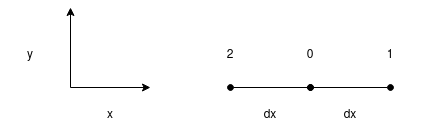
\includegraphics[width=0.8\linewidth]{rod.png}
    \caption{Test}
\end{figure}
%----------------------------------------------------------------
this leads to the values
%-----------------\left.\pdv[q]{f}{x_i}\right|_0 \approx \sum_{n = 1}^N-----------------------------------------------
\begin{table}[ht]
	\centering
    \caption{Simulation domain, rotational symmetry}
    \begin{tabular}{cccccc}
    	\hline
    	$r_1$ & $r_2$ & $N$ & $\hat{w}_n$ & $q_1$ & $q_2$ \\
    	\hline\hline
    	$\Delta x$ & $-\Delta x$ & \num{2} & $1$ & $1/\Delta x$ & $-1/\Delta x$ \\
    	\hline
    \end{tabular}
\end{table}
%----------------------------------------------------------------
\begin{equation}
	Q = q_{1} + q_{2} = \frac{1}{\Delta x} - \frac{1}{\Delta x} = 0
\end{equation}
\begin{equation}
	A = q_1\cdot \alpha_1 + q_2 \cdot \alpha_2 =  \frac{\alpha_1 - \alpha_2}{\Delta x}
\end{equation}
\begin{equation}
	\hat{A} = \frac{q_1}{r_1} \cdot \alpha_1 + \frac{q_2}{r_2} \cdot \alpha_2 =  \frac{\alpha_1  + \alpha_2}{\Delta x^2}
\end{equation}
leads to
\begin{equation}
	\alpha \cdot \nabla^2 f \approx f_1 \cdot \frac{1}{\Delta x} \cdot \left( \frac{\alpha_1}{\Delta x} - \frac{\alpha_1 - \alpha_2}{\Delta x} \right) + f_2 \cdot \frac{1}{\Delta x} \cdot \left( \frac{\alpha_2}{\Delta x} + \frac{\alpha_1 - \alpha_2}{ \Delta x} \right) - f_0 \cdot \frac{\alpha_1  + \alpha_2}{ \Delta x^2}
\end{equation}
\begin{equation}
	\alpha \cdot \nabla^2 f \approx f_1 \cdot \frac{\alpha_2}{\Delta x^2} + f_2 \cdot \frac{\alpha_1}{\Delta x^2} - f_0 \cdot \frac{\alpha_1  + \alpha_2}{ \Delta x^2}
\end{equation}

\subsection{Refined Laplace-Operator}
Text
\begin{equation}
	\left.\pdv[2]{f}{x_i}\right|_0 \approx \sum_{n = 1}^{N - 1} \sum_{k = n +1}^{N} (f'_n - f'_k) \cdot \frac{1}{2 \cdot (\vec{x}_{n, i} - \vec{x}_{k, i})} \cdot \underbrace{\frac{w_{nk}}{\sum_{n = 1}^{N - 1} \sum_{k = n +1}^{N}  w_{nk}}}_{\hat{w}_{nk}}
\end{equation}
\begin{align}
	\left.\pdv[2]{f}{x_i}\right|_0 &\approx \sum_{n = 1}^{N - 1} \sum_{k = n +1}^{N} \left(\frac{f_n - f_0}{\vec{x}_n - \vec{x}_0} - \frac{f_k - f_0}{\vec{x}_k - \vec{x}_0} \right) \cdot \underbrace{\frac{\hat{w}_{nk}}{2 \cdot (\vec{x}_{n, i} - \vec{x}_{k, i})}}_{q_{nk, i}}, \, r_{p, i} \equiv \vec{x}_p - \vec{x}_0\\
	&= \sum_{n = 1}^{N - 1} \sum_{k = n +1}^{N} (f_n - f_0) \cdot \frac{q_{nk, i}}{r_{n, i}}  - \sum_{n = 1}^{N - 1} \sum_{k = n +1}^{N}  (f_k - f_0) \cdot \frac{q_{nk, i}}{r_{k, i}} \\
	&= \sum_{n = 1}^{N - 1} \sum_{k = n +1}^{N} f_n \cdot \frac{q_{nk, i}}{r_{n, i}}  - \sum_{n = 1}^{N - 1} \sum_{k = n +1}^{N}  f_k  \cdot \frac{q_{nk, i}}{r_{k, i}} + f_0 \left( \sum_{n = 1}^{N - 1} \sum_{k = n +1}^{N} \frac{q_{nk, i}}{r_{k, i}} - \sum_{n = 1}^{N - 1} \sum_{k = n +1}^{N} \frac{q_{nk, i}}{r_{n, i}} \right)
\end{align}
leads to
\begin{multline}
	\left.\pdv[2]{f}{x_i}\right|_0 \approx \sum_{n = 1}^{N - 1} \sum_{k = n +1}^{N} f_n \cdot \frac{q_{nk, i}}{r_{n, i}}  - \sum_{n = 1}^{N - 1} \sum_{k = n +1}^{N}  f_k  \cdot \frac{q_{nk, i}}{r_{k, i}} \\
	+ f_0 \cdot \underbrace{\left( \sum_{n = 1}^{N - 1} \sum_{k = n +1}^{N} \frac{q_{nk, i}}{r_{k, i}}
	 - \sum_{n = 1}^{N - 1} \sum_{k = n +1}^{N} \frac{q_{nk, i}}{r_{n, i}} \right)}_{Q_i}
\end{multline}
Can be reformulated to
\begin{equation}
	\left.\pdv[2]{f}{x_i}\right|_0 \approx \sum_{n = 1}^{N - 1} \frac{f_n}{r_{n, i}} \sum_{k = n +1}^{N}  q_{nk, i}  - \sum_{k = 2}^{N} \frac{f_k}{r_{k, i}} \sum_{n = 1}^{k - 1}  q_{nk, i} + f_0 \cdot Q_i
\end{equation}
